\documentclass{beamer}

\usetheme{default}
\setbeamercolor{background canvas}{bg=white}
\setbeamercolor{structure}{fg=black}
\setbeamercolor{normal text}{fg=black}
\setbeamertemplate{navigation symbols}{}
\setbeamertemplate{footline}{}

% Small grey image credit, placed directly under a figure.
\newcommand{\credit}[1]{\par\vspace{0.3em}{\tiny\color{gray}#1}}

\begin{document}

\begin{frame}
  \begin{center}
    {\LARGE Welcome to}\\[1em]
    {\LARGE ASEN 3502}\\[0.5em]
    {\LARGE Computational Methods}
  \end{center}
\end{frame}

\begin{frame}{Apollo 13}
  \begin{columns}[T]
    \begin{column}{0.52\textwidth}
      \centering
      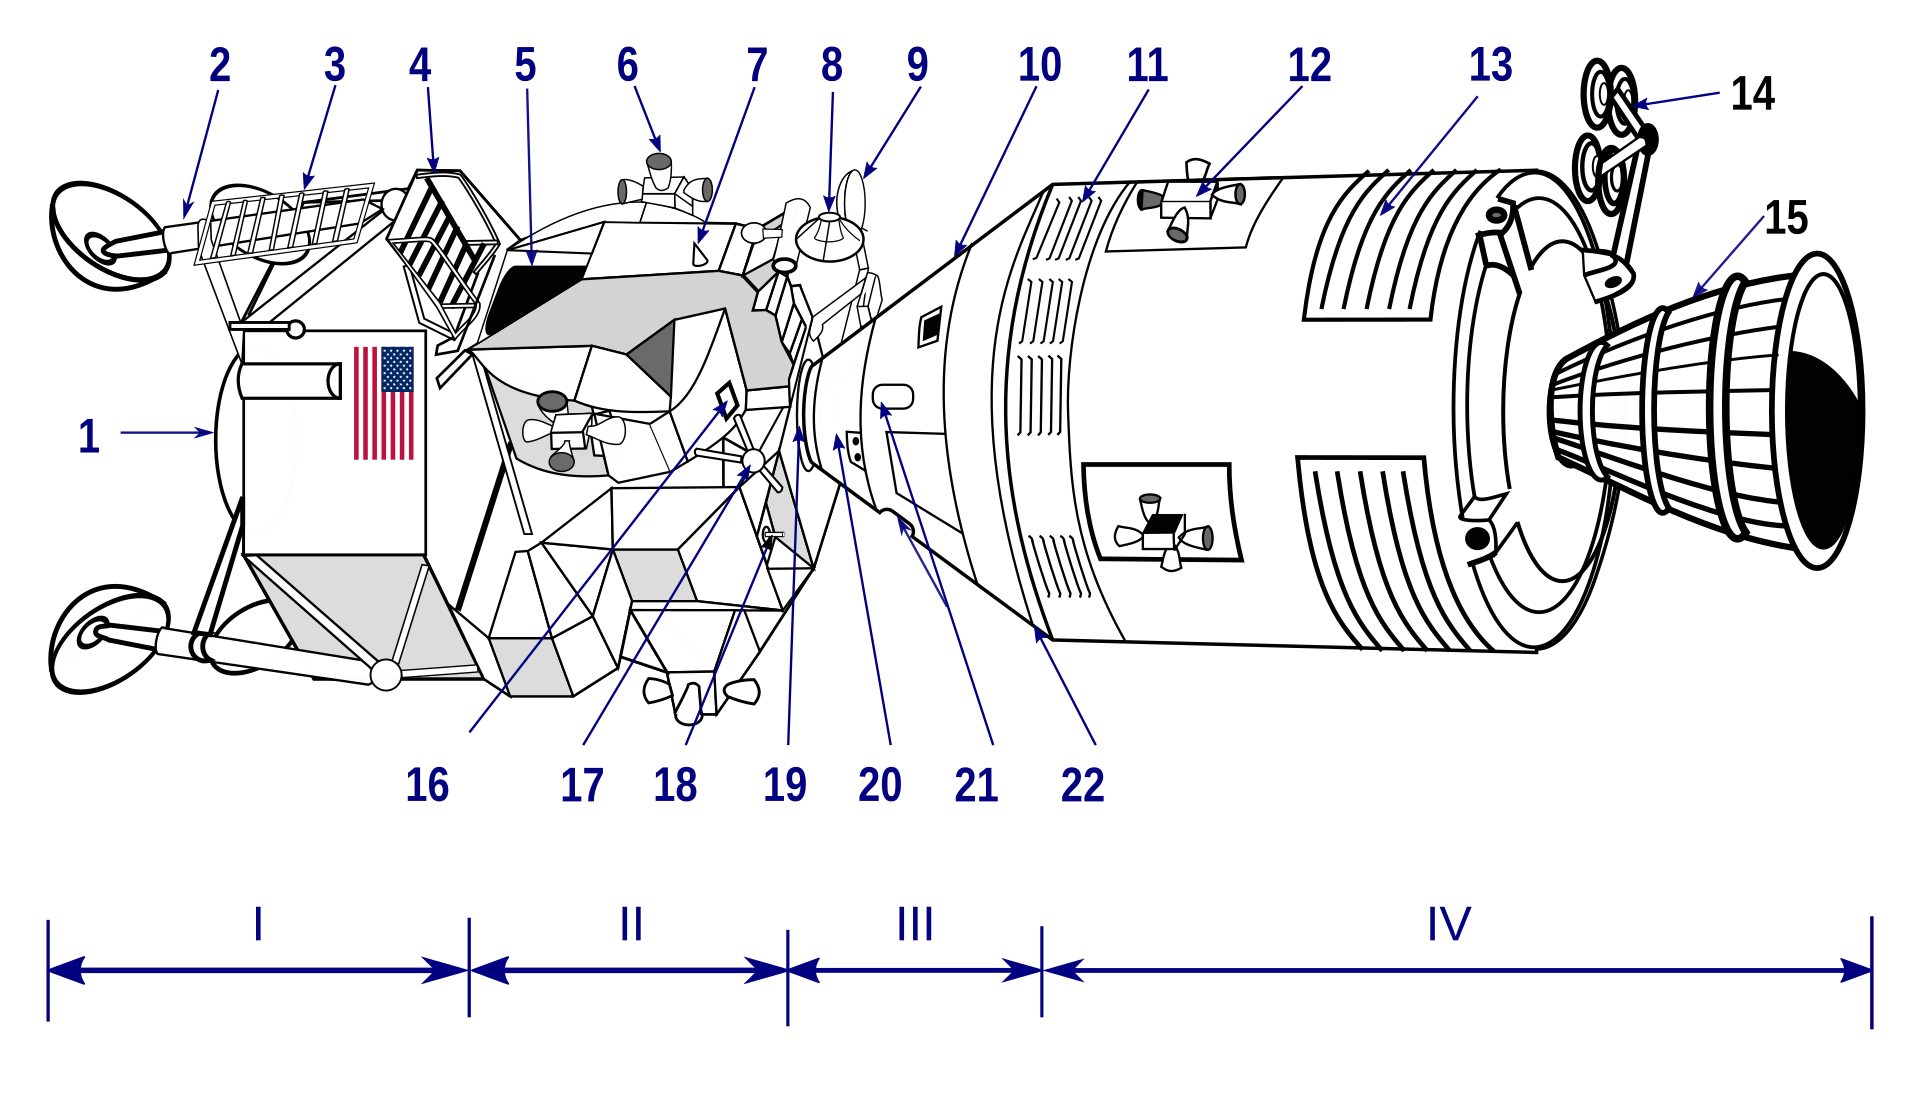
\includegraphics[width=\linewidth]{apollo-csm-lm-diagram.png}
      \credit{I--II: lunar module (descent, ascent stages);
        III: command module; IV: service module.\\
        Popadius, Wikimedia Commons, CC0.}
    \end{column}
    \begin{column}{0.44\textwidth}
      \centering
      \onslide<2->{%
        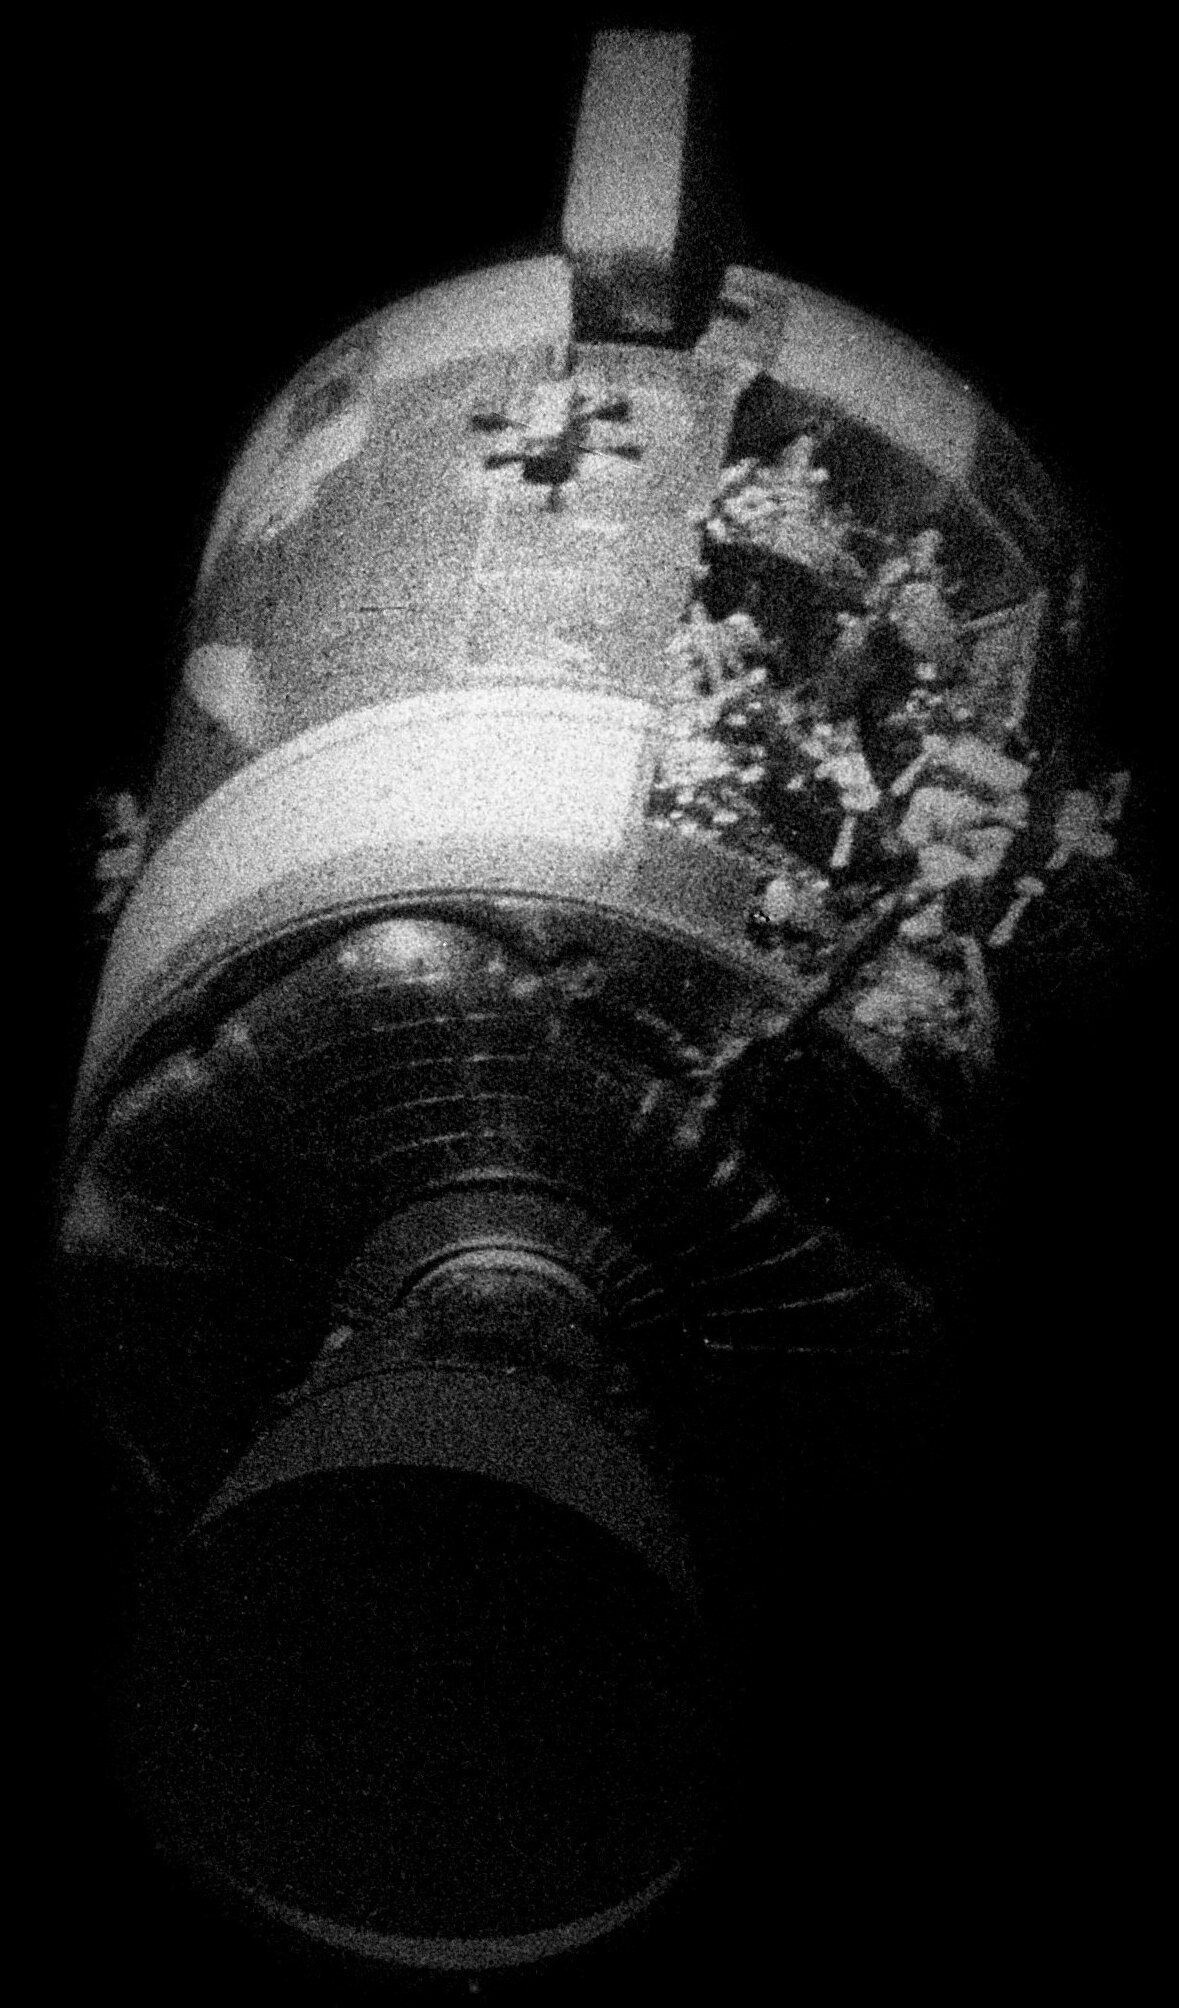
\includegraphics[height=0.62\textheight]{apollo-sm-damage.jpg}
        \credit{The service module after separation, with one panel
          blown off. NASA (scan by Kipp Teague), public domain.}%
      }
    \end{column}
  \end{columns}
\end{frame}

\begin{frame}{Direct return}
  \begin{center}
    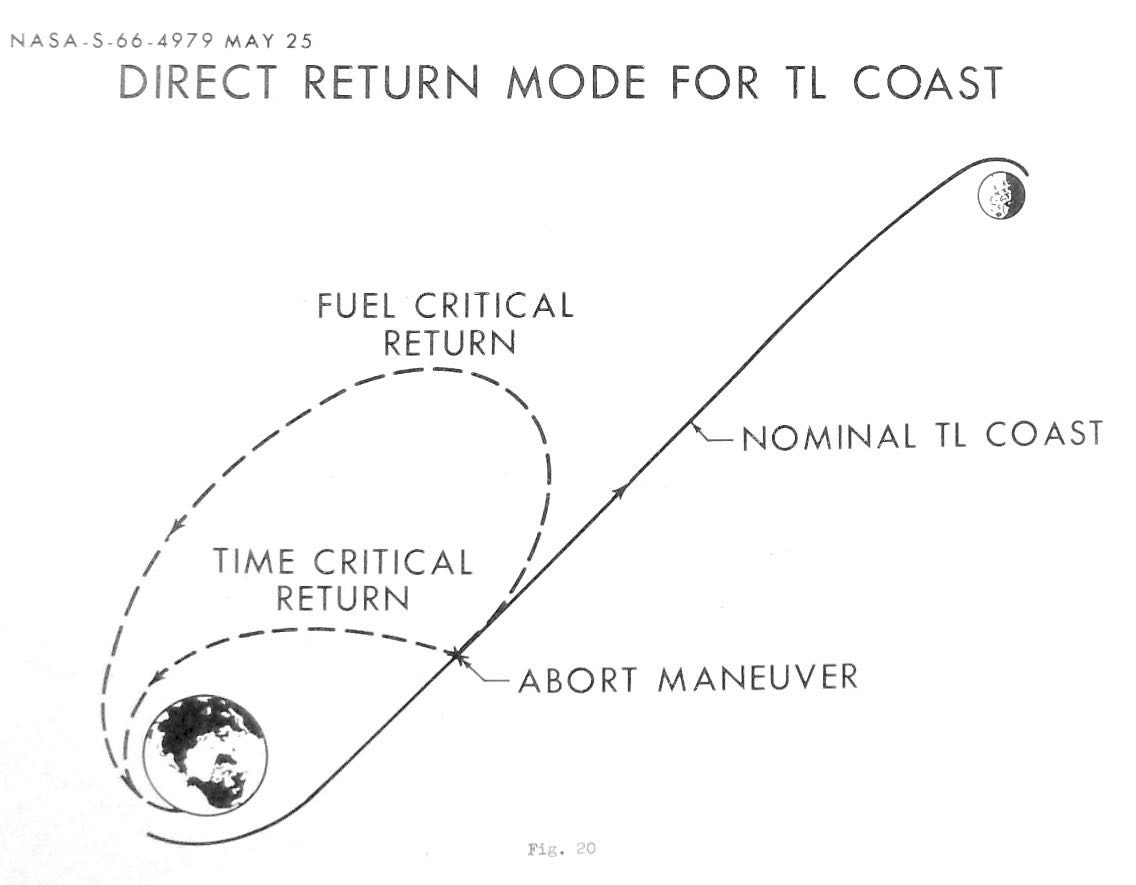
\includegraphics[height=0.78\textheight]{apollo-direct-abort.jpg}
    \credit{R.\ L.\ Berry, \emph{Apollo Lunar Landing Mission Symposium},
      NASA MSC, June 1966. Public domain, via Wikimedia Commons.}
  \end{center}
\end{frame}

\begin{frame}{What Apollo 13 actually flew}
  \begin{center}
    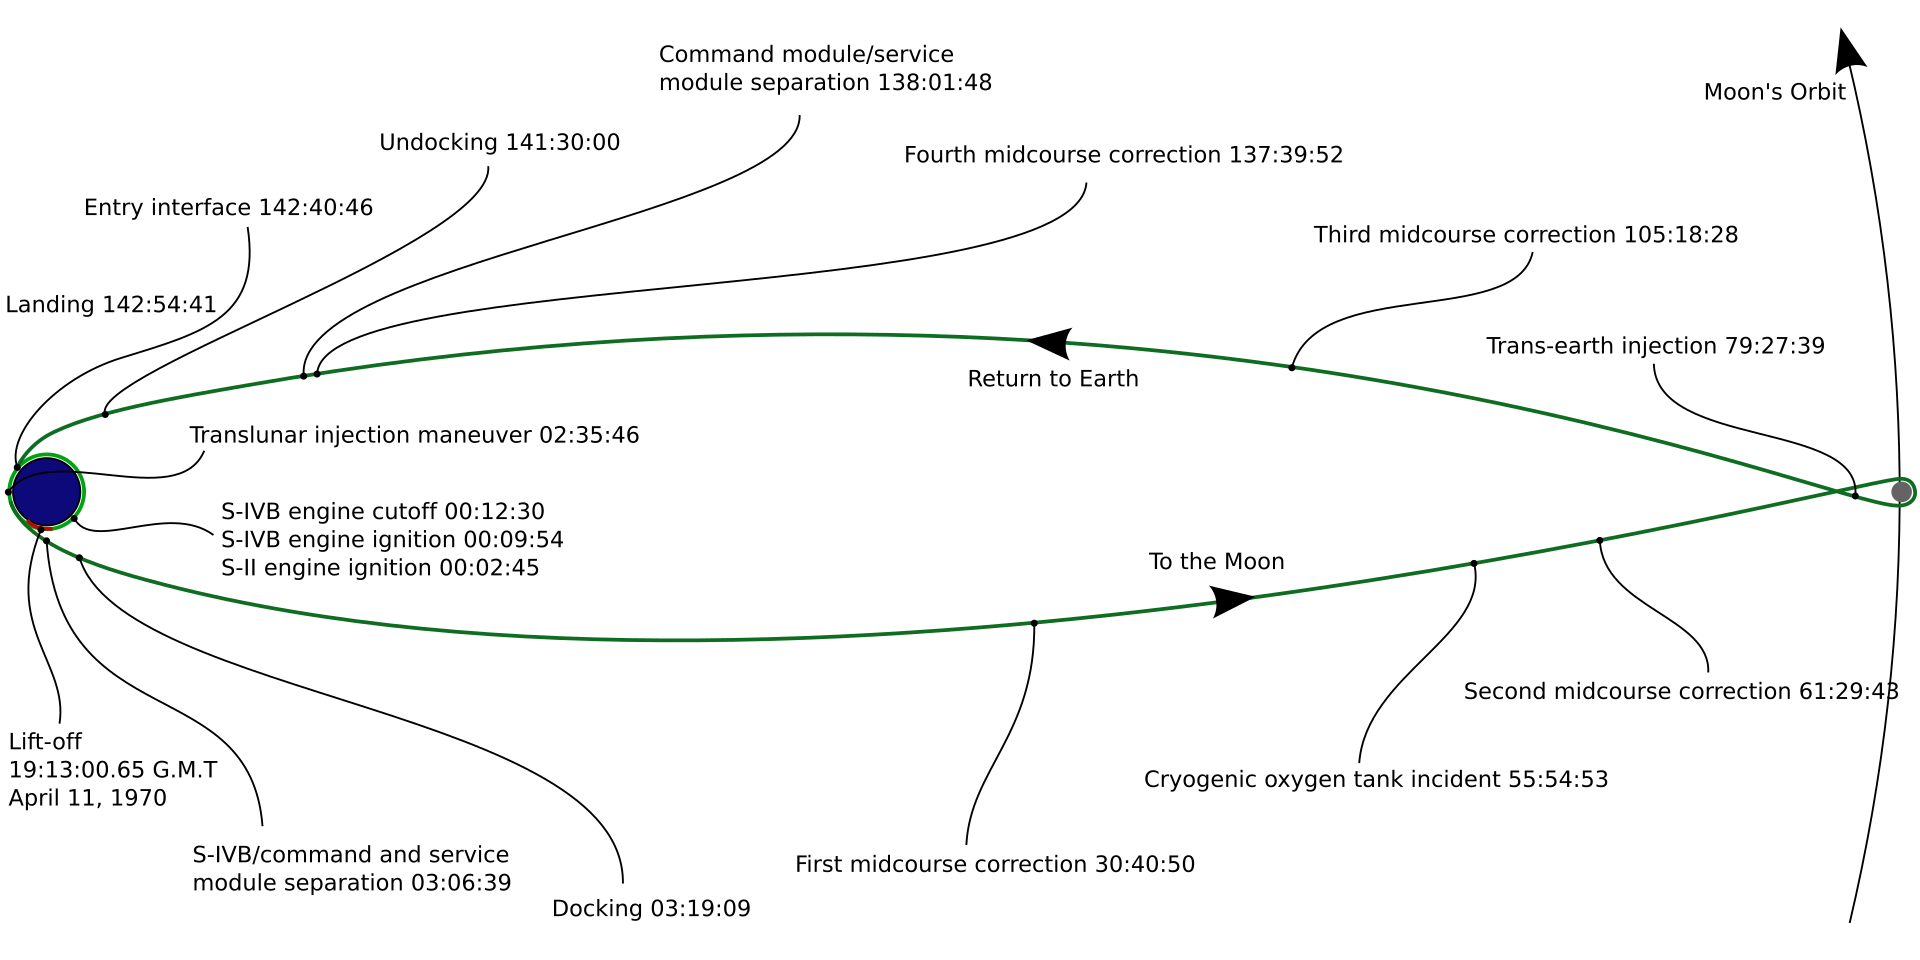
\includegraphics[width=\linewidth]{apollo13-timeline.png}
    \credit{AndrewBuck, Wikimedia Commons, CC BY-SA 4.0.
      Source for figures: Apollo 13 Mission Report, p.~3-2.}
  \end{center}
\end{frame}

\begin{frame}{ASME V\&V 10}
  \begin{columns}[c]
    \begin{column}{0.48\textwidth}
      \centering
      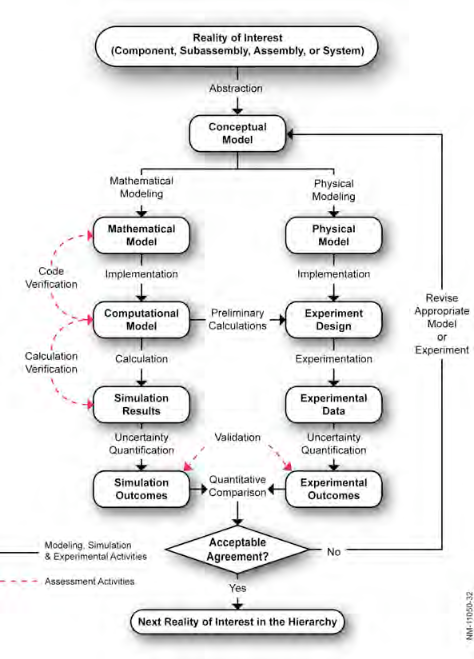
\includegraphics[width=\linewidth]{vnv.png}
    \end{column}
    \begin{column}{0.48\textwidth}
      \centering
      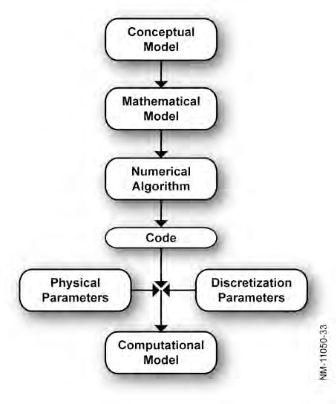
\includegraphics[width=\linewidth]{computational-model.png}
    \end{column}
  \end{columns}
  \credit{ASME V\&V 10, \emph{Guide for Verification and Validation in
    Computational Solid Mechanics}.}
\end{frame}

\begin{frame}
  \begin{center}
    {\Huge\bf asen3502.com}
  \end{center}
\end{frame}

\begin{frame}{Our Assumptions}
  \begin{columns}[c]
    \begin{column}{0.58\textwidth}
      \small
      \begin{itemize}[<+->]\setlength{\itemsep}{0.3em}
        \item The material is challenging, and can take multiple engagements to
          understand fully
        \item A student who comes to my office or asks a question wants to learn
        \item It may take multiple ways of explaining a concept before a student
          understands
        \item We must work together to help you find the way to understand
        \item Taking notes in class and doing the homework yourselves are
          critical steps to understanding
        \item I am trying to bring you to the point of understanding, not just
          give you the answer
        \item We will have fun this semester
      \end{itemize}
    \end{column}
    \begin{column}{0.40\textwidth}
      \centering
      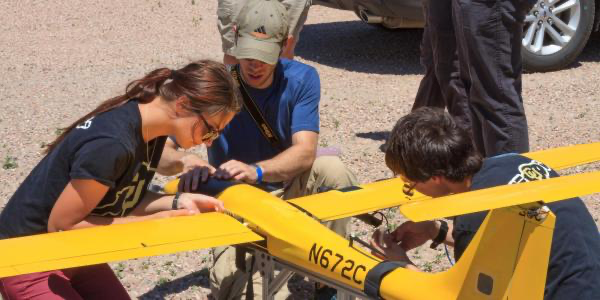
\includegraphics[width=\linewidth]{students-working-1.png}\\[1em]
      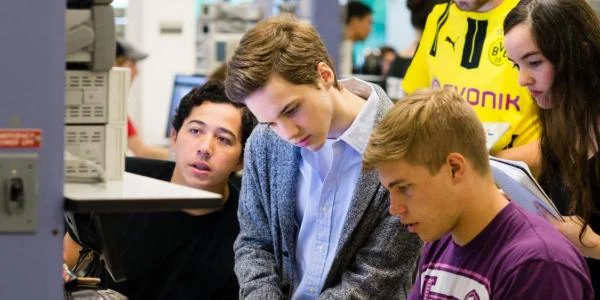
\includegraphics[width=\linewidth]{students-working-2.png}
    \end{column}
  \end{columns}
\end{frame}

\begin{frame}
\end{frame}

\end{document}
